\documentclass[exercice,a4]{thedocument}%
\usepackage{texmaths-tikz}%
\usepackage{scratch3}%
\usepackage{tabularx}%
\usepackage[np]{numprint}%
\startdatakeys
\source{24GENMATAN1}
\BO{2026}
\cycle{4}
\competencesDuSocle{CA,RA,CO}
\objectifsApprentissage{C4B3ca,C4D2ac,C4E1ab,C4E1ad,C4E1ag}
\motsCles{triangle équilatéral,Thalès,Scratch,programme,angle}
\enddatakeys
\begin{document}%
Dans cet exercice on considère la figure codée ci-contre.
\begin{itemize}
    \item Les points A, C et E sont alignés.
    \item Les points B, C et D sont alignés.
    \item $\mathrm{AB}=\np[mm]{240}$.
    \item $\mathrm{CE}=\np[mm]{80}$.
\end{itemize}

\begin{center}
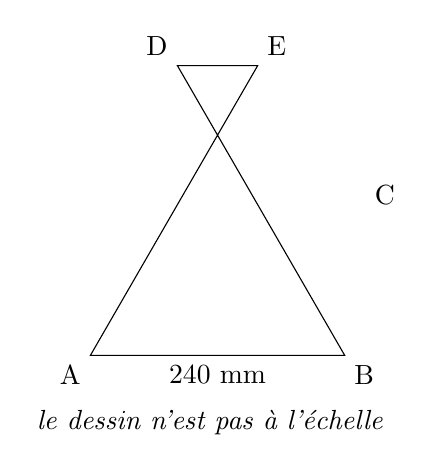
\begin{tikzpicture}[scale=.85]
    \draw (0,0) node[below left]{A}--(3.8,0) node[below right]{B}
        --++(120:5) node[above left]{D}--++(1.2,0) node[above right]{E}
        --cycle;
    \draw (0,0)--(3.8,0) node[midway,below]{240 mm};
    \node at (4.4,2.4){C};
    \node at (1.8,-1){\emph{le dessin n'est pas à l'échelle}};
\end{tikzpicture}
\end{center}

\textbf{Partie A}
\begin{enumerate}
    \item Montrer que le triangle ABC est équilatéral.
    \item Montrer que les droites (DE) et (AB) sont parallèles.
\end{enumerate}

\textbf{Partie B}

On donne le programme suivant qui permet de tracer la figure précédente. Ce
programme comporte une variable nommée « côté ». Les longueurs sont données
en pas : \textbf{1 pas représente 1 mm}.

\begin{center}
\begin{tabularx}{\linewidth}{|X|X|}\hline
\textbf{Programme} & \textbf{Le bloc triangle}\\ \hline
\begin{scratch}[num blocks,scale=.65]
    \blockinit{quand \greenflag est cliqué}
    \blockmove{aller à x : \ovalnum{-180} y : \ovalnum{-150}}
    \blockmove{s'orienter à \ovalnum{90}}
    \blockvariable{mettre \selectmenu{côté} à \ovalnum{...}}
    \blockmoreblocks{triangle}
    \blockmove{tourner \turnleft{} de \ovalnum{60} degrés}
    \blockmove{avancer de \ovalnum{240}}
    \blockvariable{mettre \selectmenu{côté} à
        \ovaloperator{\ovalvariable{côté}/\ovalnum{3}}}
    \blockmoreblocks{triangle}
\end{scratch}
&
\begin{scratch}[scale=.65]
    \initmoreblocks{définir \namemoreblocks{triangle}}
    \blockpen{stylo en position d'écriture}
    \blockrepeat{répéter \ovalnum{3} fois}{
        \blockmove{avancer de \ovalvariable{côté} pas}
        \blockmove{tourner \turnleft{} de \ovalnum{120} degrés}}
    \blockpen{relever le stylo}
\end{scratch}
\\ \hline
\end{tabularx}
\end{center}

\begin{enumerate}
    \item Quelles sont les coordonnées du point de départ du lutin ?
    Aucune justification n'est demandée.
    \item Quelle valeur doit être saisie à la ligne 4 du programme ?
    Aucune justification n'est demandée.
    \item Le lutin démarre à la case D8. Dans quelle case se trouve-t-il
    lorsqu'il vient d'exécuter la ligne 7 du programme ? Aucune justification
    n'est demandée.
\end{enumerate}

\begin{center}
\begin{tikzpicture}[x=8mm,y=8mm]
    \draw[dotted] (0,0) grid (10,-8);
    \foreach \y in {1,...,8}
        \node at(-.3,-\y+.5){\y};
    \foreach \x/\l in {1/A,2/B,3/C,4/D,5/E,6/F,7/G,8/H,9/I,10/J}
        \node at(\x-.5,.5){\l};
    \draw (3.5,-7.5)--(9.5,-7.5)--(5.5,-.5)--(7.5,-.5)--cycle;
\end{tikzpicture}
\end{center}

\begin{enumerate}
    \setcounter{enumi}{3}
    \item Expliquer l'instruction « côté $/3$ » de la ligne 8 du programme
    pour le tracé de la figure.
\end{enumerate}
\showthesource
\end{document}
